\documentclass[11pt]{article}
\usepackage{hyperref}
\usepackage[toc,page]{appendix}
\usepackage{changepage}
\usepackage{fancyvrb}
\usepackage{graphicx}
\author{Edin Jakupovic}
\title{Kafka: Delivery Guarantees}

\begin{document}
\maketitle
\clearpage


\section*{Abstract}
Messaging systems are commonly used in distributed software to pass messages between different parts of a system.
By introducing a messaging abstraction between different subsystems, systems can gain some very beneficial properties at the cost of introducing new challenges.
\newline
\newline
Passing messages between subsystems can be further complicated by running systems in a distributed manner, where the system is expected to keep working despite partial failures and without data loss.
\newline
\newline
Depending on what the purpose of the system is, delivery of messages require different guarantees. Ensuring that messages are sent and received according to some constraints can be achieved by making certain design and configuration choices. However, achieving such guarantees comes with a set of tradeoffs for each approach.
\newline
\newline
This article will discuss different design choices when implementing messaging using the messaging system Kafka, and what impact and consequence they have for the design of a distributed system. To give some concrete examples, three common delivery guarantees will be discussed and implemented using Kafka.

\clearpage
\section*{Glossary of Terms, Abbreviations and Acronyms}
\textbf{I/O} - Input/Output
\newline
\textbf{CAP} - Consistency, Availability, Partial Tolerance
\newline
\textbf{RPC} - Remote procedure call
\newline
\textbf{Asynchrony} - Occurrence of uncoordinated flows that run independent of the main program flow and don't block until completion.
\newline
\textbf{Synchrony} - Occurrence of coordinated flows that run in sequence blocking each part until completion.
\newline
\textbf{Cluster} - Set of computers that work together and can be viewed as a single system.
\newline
\textbf{Coupling} - Degree of how dependent a piece of software is on another.
\newline
\textbf{Monolithic system} - A system that performs a function within a single program on a single platform.
\newline
\textbf{Data replication} - Writing an additional copy of data in another location.
\newline
\textbf{ACK} - Acknowledgement code that is returned to callers to indicate a result from the callee.

\clearpage

\tableofcontents
\clearpage
\section{Communication within Distributed Systems}
With ever increasing requirements on scale and availability, traditional single process/machine monolithic systems are often not a good fit. Vertically scaling systems are limited in how much they can scale to accommodate traffic. Additionally, having a single point of processing creates a single point of failure. While more complex, distributed systems solve some of these problems but at the cost of a less predictable system.
\newline
\newline
By splitting a system up in independent subsystems and spreading them out over multiple processes and/or machines, parts of the system can continue running even with partial failures. Distributing a system does not give this property by itself unless partial failures are also handled by subsystems. A single machine can only scale so much until the cost and performance of parts reaches a roof. Cheap machines, while less powerful, are easier to maintain and more cost effective.
\newline
\newline
In a monolithic single process system, making a function call is expected to pretty much always execute the desired code on the CPU unless hindered by obscure OS scheduling bugs or hardware failures. This semi guarantee narrows known error handling down to implementing system logic accurately according to some desired behaviour.
\newline
\newline
Another class of errors are errors introduced when performing input/output(I/O) operations through less stable interfaces such as network cards and harddrives. These interfaces can fail unpredictably for many reasons and are unpredictable in terms of throughput.
\newline
\newline
In a distributed system, unpredictable I/O calls are far more common and unlike a single process system function call, the result of invoking a remote procedure is unknown to the caller until a response is received. This creates an issue because sub-systems only communicate through unreliable messaging.
\subsection{Synchronous Invocation - Remote Procedure}
Distributed systems can be built around the idea of remote procedure calls. Subsystems that are run in different processes or machines are treated as software modules that expose methods. In this type of synchronous communication, subsystems are invoking procedures in other sub-systems using less reliable I/O interfaces with the expectation of receiving a result once the procedure completes. This is commonly used if the result or side effect of a procedure is needed immediately after invocation.
\newline
\newline
This type of communication requires the calling system to be aware of another system's address and interface which causes tight coupling. Furthermore, invoking a RPC call requires the receiving system to be healthy and able to receive the request. After a RPC is invoked, there are 3 different outcomes the callee can expect.
\newline
\begin{itemize}
\item The RPC call is received by the target, executed and an expected response ACK is returned.
\item The RPC call is received by the target, executed and an expected error ACK is returned.
\item The RPC call fails at some point while sending or receiving data and what occurred in the sub-system is unknown.
\end{itemize}



\subsection{Asynchronous Messaging}
Another communication paradigm involves a non-waiting approach where the result of a message is not needed or desired at the time of sending. In this case, a sub-system only needs to know where to send messages, rather than to whom, which decouples the sub-system from other sub-systems. The responsibility of routing or exposing the message is instead handled by a central message broker.
\newline
\newline
Sub-systems that are interested in messages of a certain type can then consume them from the brooker at a later time without being coupled to the producer of the message. Depending on the message broker delivery system, this design also removes temporal coupling since messages can be produced without requiring an available consumer. Sending a message to a message broker still requires a synchronous invocation if we want to ensure that our message is sent. The overall availability of a system now depends on the health of the message broker instead of every sub-system which is easier to manage.

\subsection{Asynchronous vs Synchronous Communication}

Choosing a communication approach comes with various tradeoffs depending on what is required of a system. Decoupling subsystems through a messaging abstraction prevents failures in one subsystem from affecting other subsystems' ability to produce messages. As long as the broker is healthy, data can flow through the system without failures cascading up through the call chain.
\newline
\newline
The downside is that failures are not propagated to the caller since the result of processing a message is decoupled, and thus the caller does not know the result of some downstream operation after completing a call. The two trade offs thus become whatever one wants to introduce latency or lose availability.

\vspace{15pt}
\begin{figure}[htbp]
\centerline{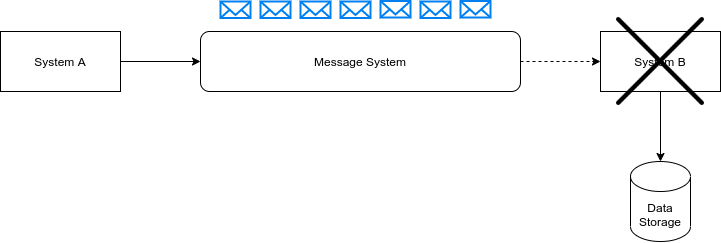
\includegraphics[scale=0.5]{assets/buffered.png}}
\caption{ Messages are buffered and will eventually be propagated but we can't detect downstream errors nor know when messages are processed.}
\label{fig}
\end{figure}

\begin{figure}[htbp]
\centerline{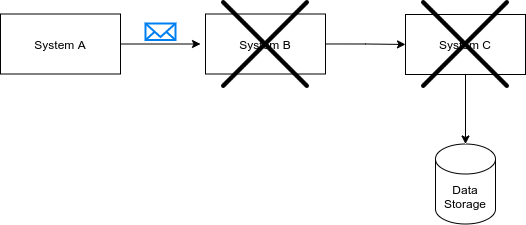
\includegraphics[scale=0.5]{assets/sync.png}}
\caption{Downstream errors get propagated to the callee and are known in synchronous systems at the cost of availability.}
\label{fig}
\end{figure}
\vspace{15pt}

If we make a RPC in a synchronous system, but a downstream dependency is unhealthy, our call gets rejected but we know it failed and can react to the failure.
If we send an asynchronous message, but a downstream consumer is unhealthy, our message will be accepted, buffered and eventually processed but at the cost of a higher latency and less knowledge.
\newline
\newline
Having to make a tradeoff between availability and consistency when persisting replicated data is a property of the CAP theorem. This theorem says that distributed systems can be either available or consistent if a network issue occurs and subsystems are unable to communicate ( Partitioned network ). Systems have to be designed around this limitation and what properties are chosen depends on the requirements of the system.


\vspace{15pt}
\begin{figure}[htbp]
\centerline{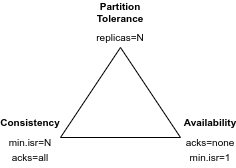
\includegraphics[scale=1]{assets/cap.png}}
\caption{ Configuring minimum in-sync replicas and number of acks can be used to tune the properties of the system.}
\label{fig}
\end{figure}
\clearpage

\section{Kafka: Messaging broker}

Kafka is a distributed messaging system. Just like most messaging systems, Kafka supports messaging through a publisher/subscriber model but has other features built on top of the basic functionality such as transforming data using Kafka Streams\cite{kafka-stream} and integrating with other systems using Kafka Connect\cite{kafka-connect}. Using Kafka effectively as a messaging abstraction requires some understanding of the underlying architecture and concepts.

\subsection{Kafka: Basic Concepts}

\subsubsection{Records ( messages/events ) }
A record is the Kafka terminology used to denote a message or also called event. Records contain both the payload and the metadata which constitute a message.

\subsubsection{Topic}
Every message sent to Kafka is sent to a specific topic. Topics are contexts under which similar messages are grouped. Topics are identified by a name and can be created ahead of time or dynamically as a message is sent containing a new topic.

\begin{figure}[htbp]
\centerline{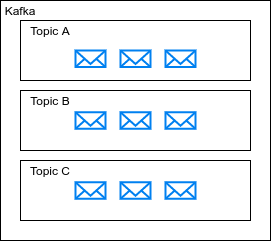
\includegraphics[scale=0.7]{assets/topics.png}}
\caption{Different topics hold different messages based on some grouping.}
\label{fig}
\end{figure}

\subsubsection{Message log}

When a message is sent to a topic, it is persisted to one or several files in an append only manner. These files represent the queues in messaging systems. These files constitute the concept of queues in messaging systems. Records are written to the end of the file and read by specifying an offset from the start of the file. Message logs are persisted on disk but can be configured to be cleaned up after a time.


\subsubsection{Partitions}
Each topic can be split into 1 or more partitions which each get a portion of the topic records. Records sent to a partition are guaranteed to be read in the same order as they were written within the partition. Messages sent to a topic can either be spread out in a round-robin manner across the partitions, or a partition key can be supplied to write to specific partitions.

\begin{figure}[htbp]
\centerline{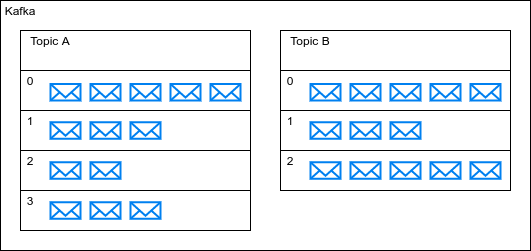
\includegraphics[scale=0.7]{assets/partitions.png}}
\caption{Topics can be further split up into partitions that are read and written too.}
\label{fig}
\end{figure}

\subsubsection{Producers}
Producers are clients that produce and push records to Kafka.

\subsubsection{Consumers}
Consumers are clients that pull records from Kafka. Consumers pull records from partitions from certain offsets. Consumers can commit an offset by persisting the offset in the Kafka cluster. If a consumer is restarted, it can read the last committed offset and continue from that record. As long as the message log persists, consumers can reread the message logs as many times they want.

\subsubsection{Consumer groups}
Consumer groups is a way of mapping N consumers to M partitions within a topic such that each message is only read by at most one consumer within the group. Consumers within a group read from the same topic but can read from multiple partitions.

\begin{figure}[htbp]
\centerline{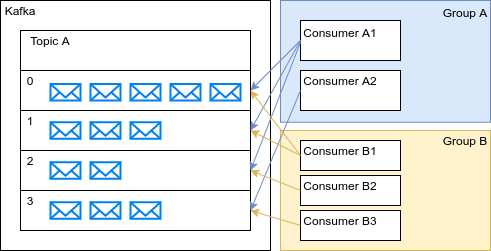
\includegraphics[scale=0.7]{assets/cgroup.png}}
\caption{Group A and B can process the same messages independently but each partition is handled by one consumer per group.}
\label{fig}
\end{figure}


\subsection{Kafka: Characteristics}
Kafka aims to be highly available and resistant to node failures when run as a distributed system. To achieve these properties, Kafka does two things, data replication and leader election.

\subsubsection{Partitioning, Availability and Durability}
In a clustered Kafka setup, every partition is replicated across to zero or more nodes based on a replication factor\cite{kafka-replication-factor}. Only one of the nodes is considered the "leader" of a particular partition\cite{kafka-replication}. A leader node receives all write operations for each partition it is responsible for. Each write to the leader is replicated to other nodes based on the replication factor.


\begin{figure}[htbp]
\centerline{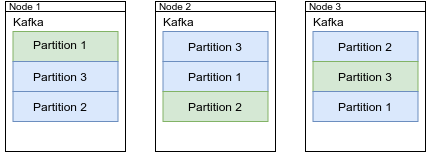
\includegraphics[scale=0.8]{assets/replication.png}}
\caption{Three node Kafka cluster where each node is leader for 1 partition marked in green with replicas in blue.}
\label{fig}
\end{figure}
Once a record has been replicated across all replicas, the record is considered committed and only then can a consumer pull it. A record is considered replicated once every replica has returned an ACK but not necessarily before the record is written to disk.
\newline
\newline
From a producer perspective, a latency/durability tradeoff can be achieved by setting the number of replicas that need to be in sync before getting an ACK on writes. As long as there is one in sync replica with a record, that record is not lost. If a replica goes down, one of the remaining healthy replicas is promoted as leader for the partitions of the failing node. Once the unhealthy node becomes healthy again, partitions can be rebalanced and reshuffled across the nodes\cite{kafka-partition-shuffling}. Increasing the replication factor does not guarantee data won't be lost but makes it less likely. If all nodes replicating a partition die, data loss can occur.
\newline
\newline
\section{Delivery Guarantees}
Depending on the requirements of a system and the desired tradeoffs, both producers and consumers can be configured for different goals. These guarantees require that only one producer is writing to a partition and only one consumer is reading at a time.

\subsection{Producer guarantees}

If a single producer sends records to a partition, they will be written in the order they are received. This ensures that the records are written in the order they were sent. This can't be guaranteed if two producers are writing to the same partition. Depending on ACK configuration, different levels of data loss can be configured.

\begin{figure}[htbp]
\centerline{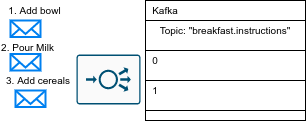
\includegraphics[scale=0.8]{assets/write.png}}
\caption{Records are written in order within a partition but not within a topic.}
\label{fig}
\end{figure}

\begin{figure}[htbp]
\centerline{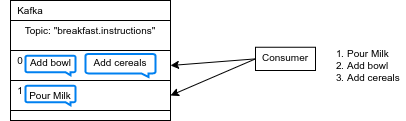
\includegraphics[scale=0.8]{assets/read.png}}
\caption{Reading from a partition only guarantees order within the partition. Wrong configuration results in instructions getting parsed out of order.}
\label{fig}
\end{figure}

\subsection{Consumer guarantees}
A consumer reading a partition will read the records in the order they were written within the partition.
As long as one in-sync replica is alive, the consumer can pull records from a partition. If a consumer fails at some point after pulling a record, they can continue reading from the last commit once they are healthy. Consumers store their offset in the Kafka cluster.
\newline
\newline
Pulling messages can have different outcomes depending on failures but there are three methods for consuming records that guarante they are processed to some degree.

\subsubsection{Processing at least once}
If a message should be processed at least once, consumers can be configured to guarantee this as long as there are remaining insync replicas. Since a consumer will always read records from the last offset it committed. 
\newline
\newline
The record from the last offset can be continuously read and attempted to process it until it succeds and can be commited. If the consumer process exits while processing a record, the last offset ensures that it will pick it up once again once healthy.

\subsubsection{Processing at most once}
If a record can't be processed more than once but it's ok if it's lost, the offset can be commited directly after reading a record but before processing it. In this case, the record will only be processed after it's commited ensuring its not processed twice.

\subsubsection{Processing exactly once}
Ensuring that a record is only processed once can be achived using only Kafka, but introduces coupling and reduced performance. Traditional way of exactly once processing requires an additional transactional system to achieve idempotency. Every time a record is produced, the producer includes a unique key. When the record is fetched, the key is used as a idempotency key to detect if a record has been processed already. The storing and processing of a record should happen in a transaction.

\clearpage
\section{Delivery guarantees Code examples}

All examples will use a single producer/consumer with the hardcoded topic "test" and partition 0.
Consumers will consume one record at a time. Code can be applied to more partitions/consumers but requires special care. The following code examples were written in Python, with Kafka deployed using docker and docker-compose.

\begin{itemize}
	\item python version: 3.8.10
	\item docker client version: 20.10.2
	\item docker server version: 20.10.2
	\item docker-compose version: 1.25.5
	\item kafka-image: confluentinc/cp-kafka:5.3.0
	\item zookeper-image: zookeeper:3.4.9
	\item{OS Linux 5.4.0-80-generic 90-Ubuntu x86\_64 GNU/Linux}
\end{itemize}

\subsection{Sending a record}
The code for sending a record will be the same across all examples. In this example we are setting ack mode to 'all' to ensure the system consistency. The program takes an argument from the terminal as a message.
\newline
\begin{adjustwidth}{-30pt}{0pt}
\begin{Verbatim}
from kafka import KafkaProducer

topic_name = "test"

servers = ['localhost:9091', 'localhost:9092', 'localhost:9093']
producer = KafkaProducer(bootstrap_servers=servers,
			 acks='all',
			 partition=0)

message = input("Enter message to send:")
producer.send(topic_name, message.encode())
producer.flush()
\end{Verbatim}
\end{adjustwidth}

\clearpage
\subsection{At Least Once}
Achieving at least once processing requires us to delay commiting the offset until we have done the processing of the record. As a result, we can process the same record multiple times if the program was to crash during or immediately after processing. But this also ensures that no record is skipped until it has been processed at least once.
\newline
\begin{adjustwidth}{-30pt}{0pt}
\begin{Verbatim}
from kafka import KafkaConsumer, TopicPartition, OffsetAndMetadata

partition = TopicPartition('test', 0)
servers = ['localhost:9091', 'localhost:9092', 'localhost:9093']
consumer = KafkaConsumer(bootstrap_servers=servers,
                       enable_auto_commit=False,
                       group_id='testgroup',
                       auto_offset_reset='earliest')
consumer.assign([partition])

result = consumer.poll(timeout_ms=3000,
                     max_records=1,
                     update_offsets=False)

if result and result[partition]:
  record = result[partition][0]
  # process record
  print("Processed record", record)
  next_offset = record.offset + 1
  consumer.commit({
      partition: OffsetAndMetadata(next_offset, None)
      })
else:
  print("No new records on partition", partition)
\end{Verbatim}
\end{adjustwidth}

\clearpage
\subsection{At most once}
At most once is similar to the "at least once" implementation except we commit the offset before we process.
\newline
\begin{adjustwidth}{-30pt}{0pt}
\begin{Verbatim}
from kafka import KafkaConsumer, TopicPartition, OffsetAndMetadata

partition = TopicPartition('test', 0)
servers = ['localhost:9091', 'localhost:9092', 'localhost:9093']
consumer = KafkaConsumer(bootstrap_servers=servers,
                       enable_auto_commit=False,
                       group_id='testgroup',
                       auto_offset_reset='earliest')
consumer.assign([partition])

result = consumer.poll(timeout_ms=3000,
                     max_records=1,
                     update_offsets=False)

if result and  result[partition]:
  record = reuslt[partition][0]
  next_offset = record.offset + 1
  consumer.commit({
              partition: OffsetAndMetadata(next_offset, None)
              })
  # process(record)
  print("Processed record ", record)
else:
      print("No new records on partition", partition)

\end{Verbatim}
\end{adjustwidth}
\clearpage
\subsection{Exactly-once}

Exactly once requires both the producer to produce at least one record but also the consumer to process it exactly once.  Doing this requires us to both persist the record in a transaction, skipping and commiting the offset. If we fail at any point while persisting, we will rollback the side effects and nothing will be committed. Using a database we can we can ensure to de-deuplicate any duplicate messages.
\newline
\begin{adjustwidth}{-30pt}{0pt}
\begin{Verbatim}
from kafka import KafkaConsumer, TopicPartition, OffsetAndMetadata
import asyncio
import asyncpg
import datetime
import json

async def main():
    conn = await asyncpg.connect(user='postgres', password='123',
                                 database='postgres', host='localhost')
    partition = TopicPartition('test', 0)
    servers = ['localhost:9091', 'localhost:9092', 'localhost:9093']
    consumer = KafkaConsumer(bootstrap_servers=servers,
                         enable_auto_commit=False,
                         group_id='testgroup',
                         auto_offset_reset='earliest')
    consumer.assign([partition])

    print("Waiting for messages..")
    for msg in consumer:
        body = msg.value.decode('utf-8')
        payload = json.loads(body)
        print("persisting", payload)
        await conn.execute('''INSERT INTO 
        				  messages(idempotency_key, message)
                          SELECT \$1, \$2 WHERE NOT EXISTS
                          ( SELECT 1 FROM messages WHERE idempotency_key = \$1)''',
                       payload['idempotency_key'],
                       payload['message'])


asyncio.get_event_loop().run_until_complete(main())
\end{Verbatim}
\end{adjustwidth}


\clearpage
Sql init code ( Postgres )
\begin{adjustwidth}{-30pt}{0pt}
\begin{Verbatim}[frame=single]
CREATE TABLE IF NOT EXISTS messages (
    id serial PRIMARY KEY,
    idempotency_key text,
    message text
);
\end{Verbatim}
\end{adjustwidth}


Updated Producer code
\begin{adjustwidth}{-30pt}{0pt}
\begin{Verbatim}
from kafka import KafkaProducer
import uuid
import json

servers = ['localhost:9091', 'localhost:9092', 'localhost:9093']
topic_name = "test"
producer = KafkaProducer(bootstrap_servers=servers, acks='all')

message = input("Enter message to send: ")
payload = {
    "idempotency_key": str(uuid.uuid4()),
    "message": message
}

p = json.dumps(payload)
producer.send(topic_name, p.encode(), partition=0)
producer.flush()
print(f'Sent {message} to topic {topic_name}')

\end{Verbatim}
\end{adjustwidth}

\clearpage

\begin{thebibliography}{9}
\bibitem{python} kafka-python library documentation
\newline
\url{https://kafka-python.readthedocs.io/en/master/index.html}

\bibitem{kafka-replication-factor} Kafka Replication Factor Property
\newline
\url{https://kafka.apache.org/documentation/#basic_ops_increase_replication_factor}

\bibitem{kafka-replication} Kafka Replication Design
\newline
\url{https://kafka.apache.org/documentation/#replication}

\bibitem{kafka} Kafka Documentation
\newline
\url{https://kafka.apache.org/documentation/}

\bibitem{kafka-stream} Kafka Streams
\newline
\url{https://kafka.apache.org/documentation/streams/}

\bibitem{kafka-connect} Kafka Connect
\newline
\url{https://docs.confluent.io/platform/current/connect/index.html}


\bibitem{kafka-partition-shuffling} Kafka Partition Rebalancing
\newline
\url{https://kafka.apache.org/documentation/#design_replicamanagment}


\end{thebibliography}

\begin{appendices}
\section*{docker-compose.yml}

\begin{adjustwidth}{-120pt}{100pt}
\begin{scriptsize}
\begin{verbatim}
version: '3'
services:
  zookeeper:
    image: zookeeper:3.4.9
    hostname: zookeeper
    ports:
      - "2181:2181"
    environment:
      ZOO_MY_ID: 1
      ZOO_PORT: 2181
      ZOO_SERVERS: server.1=zookeeper:2888:3888
    volumes:
      - ./data/zookeeper/data:/data
      - ./data/zookeeper/datalog:/datalog
  kafka1:
    image: confluentinc/cp-kafka:5.3.0
    hostname: kafka1
    container_name: kafka1
    ports:
      - "9091:9091"
    environment:
      KAFKA_ADVERTISED_LISTENERS: LISTENER_DOCKER_INTERNAL://kafka1:19091,LISTENER_DOCKER_EXTERNAL://${DOCKER_HOST_IP:-127.0.0.1}:9091
      KAFKA_LISTENER_SECURITY_PROTOCOL_MAP: LISTENER_DOCKER_INTERNAL:PLAINTEXT,LISTENER_DOCKER_EXTERNAL:PLAINTEXT
      KAFKA_INTER_BROKER_LISTENER_NAME: LISTENER_DOCKER_INTERNAL
      KAFKA_ZOOKEEPER_CONNECT: "zookeeper:2181"
      KAFKA_BROKER_ID: 1
      KAFKA_OFFSETS_TOPIC_REPLICATION_FACTOR: 1
    volumes:
      - ./data/kafka1/data:/var/lib/kafka/data
    depends_on:
      - zookeeper
  kafka2:
    image: confluentinc/cp-kafka:5.3.0
    hostname: kafka2
    container_name: kafka2
    ports:
      - "9092:9092"
    environment:
      KAFKA_ADVERTISED_LISTENERS: LISTENER_DOCKER_INTERNAL://kafka2:19092,LISTENER_DOCKER_EXTERNAL://${DOCKER_HOST_IP:-127.0.0.1}:9092
      KAFKA_LISTENER_SECURITY_PROTOCOL_MAP: LISTENER_DOCKER_INTERNAL:PLAINTEXT,LISTENER_DOCKER_EXTERNAL:PLAINTEXT
      KAFKA_INTER_BROKER_LISTENER_NAME: LISTENER_DOCKER_INTERNAL
      KAFKA_ZOOKEEPER_CONNECT: zookeeper:2181
      KAFKA_BROKER_ID: 2
    volumes:
      - ./data/kafka2/data:/var/lib/kafka/data
    depends_on:
      - zookeeper 
  kafka3:
    image: confluentinc/cp-kafka:5.3.0
    hostname: kafka3
    container_name: kafka3
    ports:
      - "9093:9093"
    environment:
      KAFKA_ADVERTISED_LISTENERS: LISTENER_DOCKER_INTERNAL://kafka3:19093,LISTENER_DOCKER_EXTERNAL://${DOCKER_HOST_IP:-127.0.0.1}:9093
      KAFKA_LISTENER_SECURITY_PROTOCOL_MAP: LISTENER_DOCKER_INTERNAL:PLAINTEXT,LISTENER_DOCKER_EXTERNAL:PLAINTEXT
      KAFKA_INTER_BROKER_LISTENER_NAME: LISTENER_DOCKER_INTERNAL
      KAFKA_ZOOKEEPER_CONNECT: "zookeeper:2181"
      KAFKA_BROKER_ID: 3
      KAFKA_OFFSETS_TOPIC_REPLICATION_FACTOR: 1
    volumes:
      - ./data/kafka3/data:/var/lib/kafka/data
    depends_on:
      - zookeeper
  kafdrop:
    image: obsidiandynamics/kafdrop
    restart: "no"
    ports:
      - "9000:9000"
    environment:
      KAFKA_BROKERCONNECT: "kafka1:19091"
    depends_on:
      - kafka1
      - kafka2
      - kafka3
  postgres:
    image: postgres:latest
    container_name: postgres
    environment:
      - POSTGRES_PASSWORD=123
      - POSTGRES_USER=postgres
      - POSTGRES_DB=postgres
      - POSTGRES_HOST_AUTH_METHOD=trust
    volumes:
      - ./sql/init.sql:/docker-entrypoint-initdb.d/init.sql
    ports:
      - "5432:5432"
   
\end{verbatim}
\end{scriptsize}

\end{adjustwidth}

\end{appendices}

\end{document}





